\section{392 --- Is Subsequence (LeetCode)}

\subsection*{Código}
\lstinputlisting{392_IsSubsequence.java}

\subsection*{Comprovante de aceite}
\begin{center}
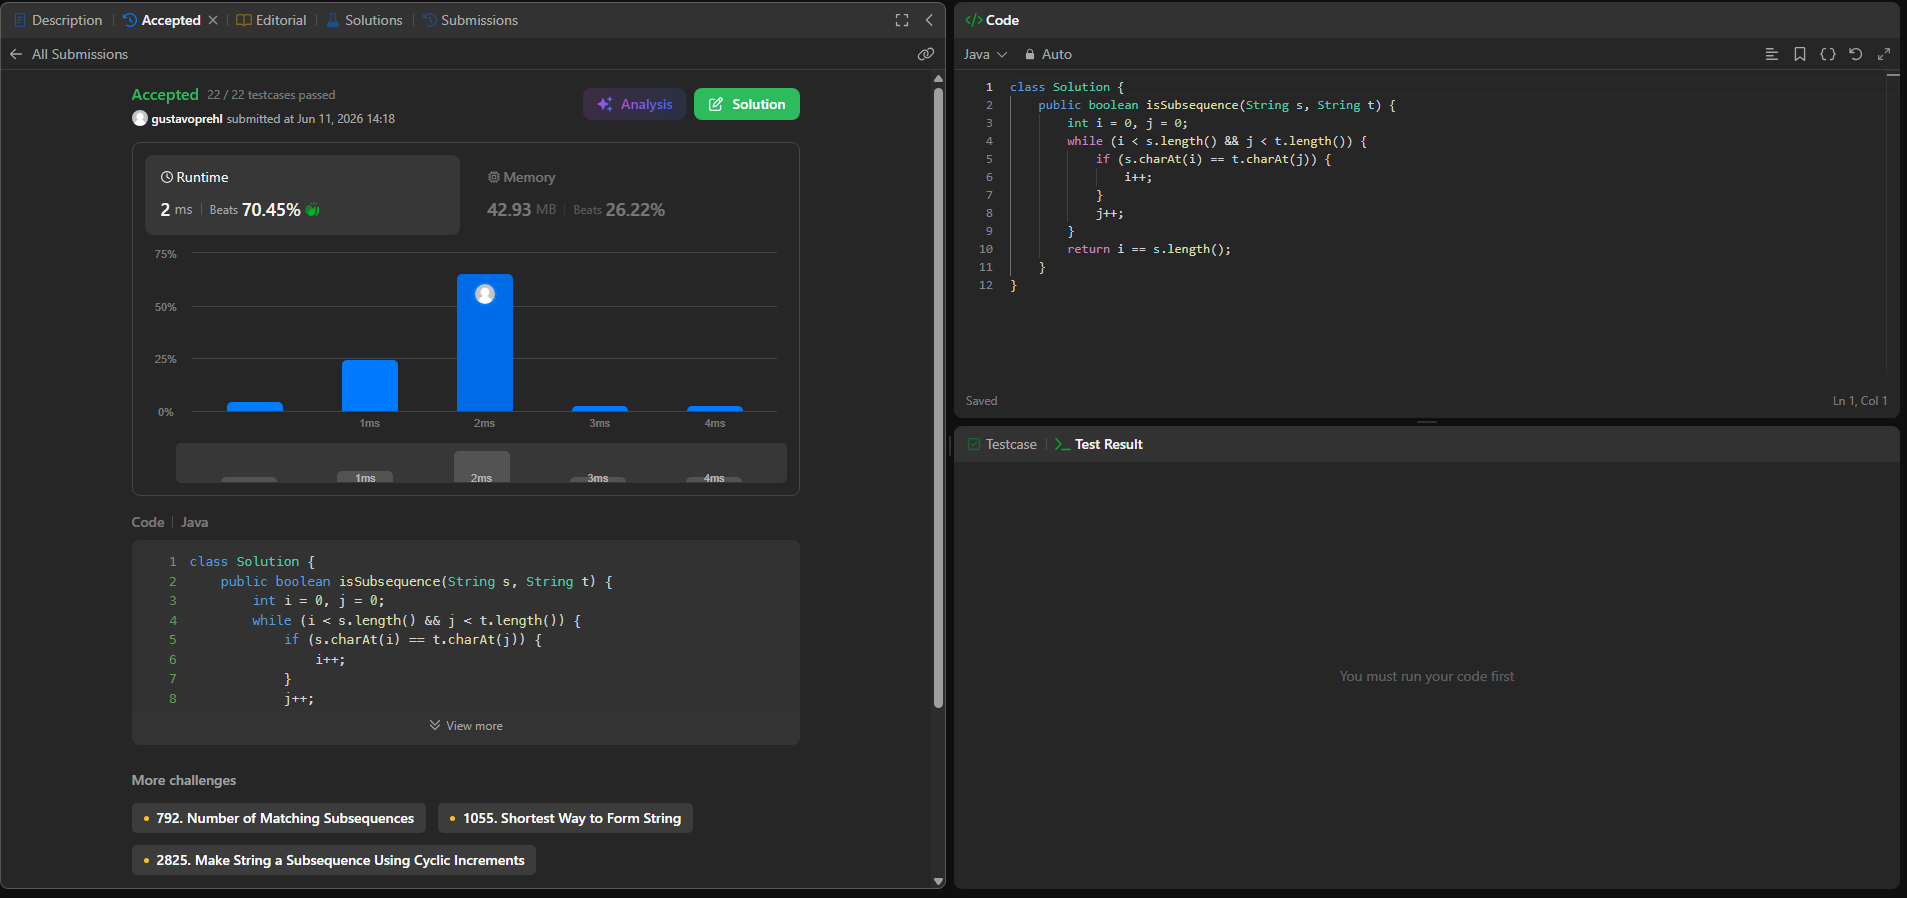
\includegraphics[width=0.85\textwidth]{Accepts/392_IsSubsequence_Submit.png}\\
\end{center}

\subsection*{Justificativa}

\textbf{Estratégia:} dois ponteiros (técnica gulosa).

A solução percorre \texttt{s} (ponteiro \texttt{i}) e \texttt{t} (ponteiro
\texttt{j}) simultaneamente. Sempre que \texttt{s[i] == t[j]}, o caractere de
\texttt{s} é ``consumido'' (\texttt{i++}); o ponteiro \texttt{j} avança a cada
iteração, independentemente de ter havido correspondência. \texttt{s} é
subsequência de \texttt{t} se, ao final, \texttt{i} percorreu todos os
caracteres de \texttt{s}.

\textbf{Por que essa escolha gulosa é ótima (correção):} dado um caractere
\texttt{s[i]} e a primeira ocorrência possível dele em \texttt{t} a partir da
posição \texttt{j}, casar \texttt{s[i]} com essa primeira ocorrência nunca é
pior do que casá-lo com uma ocorrência posterior. Isso porque qualquer
correspondência válida para o restante de \texttt{s} que use uma posição
$j' > j$ também é válida (ou mais restrita) se usarmos $j$, já que sobra mais
``espaço'' em \texttt{t} à direita. Portanto, a escolha gulosa de avançar
assim que há correspondência preserva a existência de uma solução completa,
sem necessidade de backtracking. Esse argumento de troca (\emph{exchange
argument}) é a técnica padrão de prova de corretude de algoritmos gulosos.

\textbf{Complexidade:}
\begin{itemize}
    \item Tempo: $O(|t|)$, pois cada ponteiro avança no máximo $|t|$ vezes.
    \item Espaço: $O(1)$, apenas dois índices inteiros.
\end{itemize}

\textbf{Follow-up ($k \geq 10^9$ consultas sobre o mesmo \texttt{t}):}
pré-processar \texttt{t} uma única vez, construindo, para cada caractere
\texttt{c}, a lista ordenada \texttt{pos[c]} com os índices onde \texttt{c}
ocorre em \texttt{t} --- $O(|t|)$. Para cada nova string $s_i$, percorrer seus
caracteres e, para cada um, fazer busca binária em \texttt{pos[c]} pela menor
posição estritamente maior que a posição atual em \texttt{t}. Se não existir
tal posição para algum caractere, $s_i$ não é subsequência. Isso reduz o
custo por consulta de $O(|t|)$ para $O(|s_i| \cdot \log |t|)$, o que é
essencial quando \texttt{t} é fixo e há um número muito grande de consultas.

\textbf{Tópico do curso:} estratégia gulosa, com prova de corretude por
argumento de troca --- \emph{Estratégia Gulosa e Divisão e Conquista}
[CLRS09, caps. 4 e 16].
